\section{Mining Android vulnerabilities}

In this section, we specify what data is needed for our study, how we obtained the Android vulnerability data and finally describe the data acquired.

\subsection{Acquiring the data}
\label{section:mining-acquiring}

% Data we need
For both the empirical study that assess the effectiveness of previous automatic repair tools and the purposes of devising new targeted search spaces, we need the following information for each of Android vulnerabilities:
\begin{itemize}
    %\item Description: what is the nature of a vulnerability?
    \item Patch: code before and after fixing a vulnerability
    \item Type: privilege escalation, denial of service, etc.
    \item The entire project source code before a fix (needed to assess the GenProg search space)
    \item Miscellaneous: date, severity, etc.
\end{itemize}

%Patch is the most essential part as it is required for verifying whether a patch is the search space of previous techniques and for obtaining a better understanding of vulnerability fixes. A vulnerability type is later used to 

% Where's from
The required data was obtained from the Android Security Bulletins (ASB) website\footnote{http://source.android.com/security/bulletin/}, which is the official website that lists security vulnerabilities on Android, their description and links to corresponding software repositories that contain fixes.

% How we obtained it
% Manual refinement
We created a program-crawler to parse the ASB website and organize it in a database for further use. The source code of the crawler is released\footnote{https://github.com/last5bits/cs858/tree/master/VulnCrawler}. Due to imperfections of the implementation and format inconsistencies of the website, we manually refined the data by fixing some of the fields in database (minor changes: amount of work is approximately 0.5 person-hours).

\subsection{Data description}

We mined all the data the ASB website contained at the time of running the program-crawler: 636 CVEs (the Common Vulnerability and Exposures identifications) that correspond to 251 Android vulnerabilities (the ASB website is structured in such a way that one ``vulnerability'' can correspond to multiple CVEs). Developer patches correspond to CVEs rather then ``vulnerabilities'' (using the ASB terminology); due to that, during the subsequent manual examination, we consider each CVE patch an atomic unit (rather than collection of all the CVE patches for a particular vulnerability). Later in the paper, we use the terms ``CVE'' and ``vulnerability'' interchangeably. %we use the term ``vulnerability'' to imply ``CVE''.

% No code
The most recent vulnerabilities do not have a corresponding link to the developer patch (as we suspect, due to security reasons). After removing such entries, \numvuln vulnerabilities remained, with publishing date ranging from August 2015 to August 2016.

% Severity, types, languages
The vulnerabilities obtained span several programming languages: C, C++ and Java. As Fig.~\ref{figure:severity} depicts, most of them either of a critical or a high severity. Fig.~\ref{} presents the vulnerability types. \todo{}

\begin{figure}
    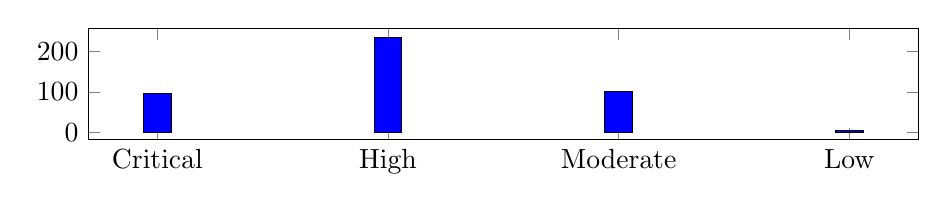
\begin{tikzpicture}
        \begin{axis}[
            symbolic x coords={Critical, High, Moderate, Low},
            xtick=data,
            height=3cm,
            width=\linewidth
          ]
            \addplot[ybar,fill=blue] coordinates {
                (Critical,   95)
                (High,  235)
                (Moderate,   100)
                (Low,   4)
            };
        \end{axis}
    \end{tikzpicture}
    \small \caption{Distribution of vulnerabilities by severity}
        \label{figure:severity}
    \vspace{-0.2in}
\end{figure}
